\documentclass{article}
\usepackage{tcolorbox, varwidth} % Boxes
\usepackage{amsthm} % For the proof environment
\usepackage{tikz}
\usepackage{graphicx}
\usepackage{xcolor}
\usepackage{float}
\usepackage{caption}
\usepackage{subcaption}
\usepackage{url}
\usepackage{geometry}
  \geometry{
 a4paper,
 total={170mm,257mm},
 left=20mm,
 top=20mm,
 }
 %
\tcbuselibrary{breakable}
\tcbuselibrary{theorems}
\tcbuselibrary{skins}

% Colours
\definecolor{faintpink}{rgb}{1,0.95,0.95}
\definecolor{TheoremColor}{RGB}{34,139,34} % Green
\definecolor{DefColor}{RGB}{45, 52, 151} % Blue
\definecolor{CorollaryColor}{RGB}{158, 80, 143} % Purple
\definecolor{ExampleColor}{RGB}{226,135,67} % Orange
\definecolor{ProofColor}{RGB}{0,177,160} % Aqua
\definecolor{NoteColor}{RGB}{158, 80, 143}
% Acronames
\usepackage[automake,acronym]{glossaries-extra}
\setabbreviationstyle[acronym]{long-short}
%--------------------------------------------------------------------------------------------
\newacronym{em}{EM}{Electro-Magnetic}
\newacronym{lhs}{LHS}{Left Hand Side}
\newacronym{wrt}{w.r.t}{with respect to}
\newacronym{rhs}{CFT}{Right Hand Side}
\newacronym{eom}{E.O.M}{Equation of Motion}
\newacronym{dbc}{D.B.C}{Dirichlet Boundary Conditions}
\newacronym{nbc}{N.B.C}{Neumann Boundary Conditions}
\makeglossaries
%-----------------------------------------------------------------------------------------
\newtcbox{\highlightbox}{nobeforeafter, colframe=black!40, colback=pink!10,
  boxrule=0.4pt, boxsep=2pt, arc=0pt, left=1pt, right=1pt, top=1pt, bottom=1pt}
  
\usepackage{calligra}
\DeclareMathAlphabet{\mathcalligra}{T1}{calligra}{m}{n}
\DeclareFontShape{T1}{calligra}{m}{n}{<->s*[2.2]callig15}{}

% Lowercase curly r in math mode
\newcommand{\scriptr}{\mathord{\mathcalligra{r}}}
\newcommand{\boldscriptr}{\mathord{\pmb{\mathcalligra{r}}}}
%--------------------------------------------------------------------------------------------
%Section
\newcommand{\lecture}[1]{
  \section{Lecture \thesection: #1}
}
% Theorem
\newtcbtheorem[number within = section]{theorem}{Theorem}%
{enhanced,frame empty,interior empty,colframe=TheoremColor!50!white,
	coltitle=TheoremColor!50!black,fonttitle=\bfseries,colbacktitle=TheoremColor!15!white,
	borderline={0.5mm}{0mm}{TheoremColor!15!white},
	borderline={0.5mm}{0mm}{TheoremColor!50!white,dashed},
	attach boxed title to top center={yshift=-2mm},
	boxed title style={boxrule=0.4pt},varwidth boxed title}{theo}

% Definition
\newtcbtheorem[number within = section]{definition}{Definition}%
{enhanced,frame empty,interior empty,colframe=DefColor!50!white,
	coltitle=DefColor!50!black,fonttitle=\bfseries,colbacktitle=DefColor!15!white,
	borderline={0.5mm}{0mm}{DefColor!15!white},
	borderline={0.5mm}{0mm}{DefColor!50!white,dashed},
	attach boxed title to top center={yshift=-2mm},
	boxed title style={boxrule=0.4pt},varwidth boxed title}{defo}

% Corollary
\newtcbtheorem[number within = section]{corollary}{Corollary}%
{enhanced,frame empty,interior empty,colframe=CorollaryColor!50!white,
	coltitle=CorollaryColor!50!black,fonttitle=\bfseries,colbacktitle=CorollaryColor!15!white,
	borderline={0.5mm}{0mm}{CorollaryColor!15!white},
	borderline={0.5mm}{0mm}{CorollaryColor!50!white,dashed},
	attach boxed title to top center={yshift=-2mm},
	boxed title style={boxrule=0.4pt},varwidth boxed title}{defo}

% Example
\newtcbtheorem[number within = section]{example}{Example}%
{enhanced,frame empty,interior empty,colframe=ExampleColor!50!white,
	coltitle=ExampleColor!50!black,fonttitle=\bfseries,colbacktitle=ExampleColor!15!white,
	borderline={0.5mm}{0mm}{ExampleColor!15!white},
	borderline={0.5mm}{0mm}{ExampleColor!50!white,dashed},
	attach boxed title to top center={yshift=-2mm},
	boxed title style={boxrule=0.4pt},varwidth boxed title}{defo}

% Proof
\tcolorboxenvironment{proof}{% `proof' from `amsthm'
	blanker,breakable,left=5mm,
	before skip=10pt,after skip=10pt,
	borderline west={1mm}{0pt}{ProofColor!50!white}}

% Note
\newtcolorbox{note}[1][]{
  enhanced,
  frame empty,
  interior empty,
  colframe=NoteColor!50!white,
  coltitle=NoteColor!50!black,
  fonttitle=\bfseries,
  colbacktitle=NoteColor!15!white,
  borderline={0.5mm}{0mm}{NoteColor!15!white},
  borderline={0.5mm}{0mm}{NoteColor!50!white,dashed},
  attach boxed title to top center={yshift=-2mm},
  boxed title style={boxrule=0.4pt},
  varwidth boxed title,
  title={Note},
  #1
}

%--------------------------------------------------------------------------------------------
\begin{document}
%-----------------------------------------------------------------------------------------
\begin{titlepage}
    \begin{center}
    \vspace{0.4cm}
    \hrule
    \Huge
    \vspace{0.8cm}
        \textcolor{blue}{\textbf{Lecture Notes on Electromagnetic Theory: PHSY 603 - NISER}}
        \vspace{0.8cm}
        \hrule
        \vspace{1cm}
        \Large
        \textcolor{purple}{\textbf{Instructor : Dr. V Ravi Chandra  \\ Documented \& Edited by : Kazi Abu Rousan}}\\
        \vspace{0.5cm}
        \large
        \emph{National Institute of Science Education and Research, Bhubaneswar}\\
        %\\
        \vspace{0.8cm}
        
        \begin{center}
		\vspace{0.2cm}
		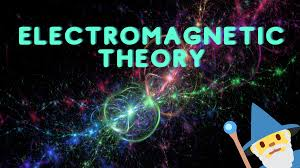
\includegraphics[height=8cm]{Images/logo.jpeg}\\
		\end{center}
        \vspace{0.5cm}
        \vspace{0.4cm}
        \Large
        Class Notes\\
        \vspace{0.7cm}
        rousan@niser.ac.in\\
      
        \vspace{1.3cm}
        
        
        
    \end{center}
\end{titlepage}
\newpage

\tableofcontents \thispagesty\dle{empty}
\pagebreak
%-----------------------------------------------------------------------------------
\lecture{Review of Electrostatics \& Magneto-statics : Maxwell's Equations}
\subsection{Motivation of studying Electrodynamics}
\textbf{Why do we need to learn this topic?}\\
Why do we learn electrodynamics?, \textbf{To explain some experiment?}, well we don't have to go that way. Just \textbf{look}...\\
Well, how will you explain this \textbf{looking} or \textbf{seeing}?\\
The answer this that \textbf{Light} reflects from different objects and then fall into our eyes, which then \textbf{excites} our \textbf{rod} and \textbf{cone} cells. How does this simulation happens?, using \textbf{Electro-Magnetic} simulation, i.e., some type of change in \textbf{voltage} and which changes the \textbf{ions} density or maybe make them move.
\begin{figure}[H]
    \centering
    \begin{subfigure}{0.4\textwidth}
        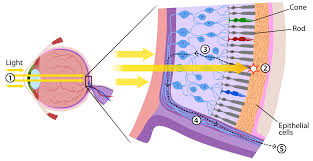
\includegraphics[width=0.9\textwidth]{Images/seeing.jpeg}
        \caption{Eyes working}
        \label{f1a}
    \end{subfigure}
    \hfill
    \begin{subfigure}{0.4\textwidth}
        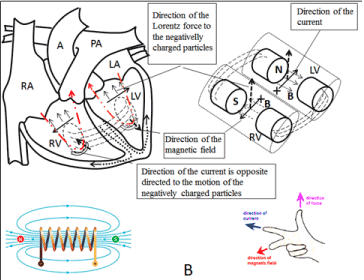
\includegraphics[width=0.7\textwidth]{Images/Heart.png}
        \caption{Heart and it's fields}
        \label{f1b}
    \end{subfigure}
    \caption{Electromagnetism working in our body.}
    \label{fig:EM_example}
\end{figure}

The heart also works using \textbf{charges}. Assume a \textbf{heart cell}, which are $10$micron in size. The cell contains $-80mV$ inside. The electric field points from outside to inside. Now, from above of the cell, the polarization changes, i.e., upper part has $20mv$ and lower has \textbf{negative charge}, creating a dipole. After some time the cell inside become totally positive. This \textbf{depolarization} waves creates the contraction and expansion of heart.\\
So, we see, \gls{em} Theory is not just important to understand "\textbf{physical experiments}" but also is important to understand the human body.

The heart also works using \textbf{charges}. Assume a \textbf{heart cell}, which are $10$micron in size. The cell contains $-80mV$ inside. The electric field points from outside to inside. Now, from above of the cell, the polarization changes, i.e., upper part has $20mv$ and lower has \textbf{negative charge}, creating a dipole. After some time the cell inside become totally positive. This \textbf{depolarization} waves creates the contraction and expansion of heart.\\
So, we see, \textbf{Electromagnetic Theory} is not just important to understand "\textbf{physical experiments}" but also is important to understand the human body.

\subsection{Maxwell's Equations}
We have studied the EM theory and how everything boils down to Maxwell's four equations. They contains all information related to EM theory. Let's see on case of \textbf{time independent} $\rho$ and $\vec{J}$ how we get the maxwell's equation using standard electrostatic and magnetostatic expressions.

As we know $\vec{E}(\vec{r})$ and $\vec{B}(\vec{r})$ are given by,
\begin{equation}
\vec{E}(\vec{r}) = \frac{1}{4\pi \epsilon_0} 
\int_{\mathcal{V}} \frac{\rho(\vec{r}')\hat{\scriptr}}{\scriptr^2} \, d\tau' = \frac{1}{4\pi \epsilon_0} 
\int_{\mathcal{V}} \frac{\rho(\vec{r}')\hat{\scriptr}}{\scriptr^2} \, d^3r'
\label{estat1}
\end{equation}
\begin{equation}
\vec{B}(\vec{r}) = \frac{\mu_0}{4\pi} 
\int_{\mathcal{V}} \frac{\vec{J}(\vec{r}')\times \hat{\scriptr}}{\scriptr^2} \, d\tau' = \frac{\mu_0}{4\pi} 
\int_{\mathcal{V}} \frac{\vec{J}(\vec{r}')\times \hat{\scriptr}}{\scriptr^2} \, d^3r'
\label{mstat1}
\end{equation}
Here $\vec{r}$ is the position where we want to find the field and $\vec{r}'$ is the source point. Also, $\vec{r}-\vec{r}'=\vec{\scriptr}$ (exactly same as griffith's book).

Using this two along with,
\begin{equation}
    \vec{F}=q(\vec{E}+\vec{v}\times \vec{B})
    \label{lorentz1}
\end{equation}
Lorentz force equation(eqn-\ref{lorentz1}), we can find forces and hence trajectory of charge particle $q$.

Using this, we get,
\begin{equation}
    \begin{split}
        \vec{\nabla}\cdot \vec{E}(\vec{r}) & = \vec{\nabla}\cdot \frac{1}{4\pi \epsilon_0} 
\int_{\mathcal{V}} \frac{\rho(\vec{r}')\hat{\scriptr}}{\scriptr^2} \, d^3r' = \frac{1}{4\pi \epsilon_0} 
\int_{\mathcal{V}}\rho(\vec{r}') \vec{\nabla}\cdot \Bigg(\frac{\hat{\scriptr}}{\scriptr^2}\Bigg) \, d^3r'\\ 
& = \frac{1}{4\pi \epsilon_0} 
\int_{\mathcal{V}}\rho(\vec{r}') 4\pi \delta^3(\vec{r}-\vec{r}') \, d^3r' = \frac{\rho(\vec{r})}{\epsilon_0} \, \, \text{ using }\vec{\nabla}\cdot \Bigg(\frac{\hat{\scriptr}}{\scriptr^2}\Bigg)=4\pi \delta^3(\vec{r}-\vec{r}')
    \end{split}
\label{gauss_1}
\end{equation}
Similarly,
\begin{equation}
    \begin{split}
        \vec{\nabla}\times \vec{E}(\vec{r}) & = \vec{\nabla}\times \frac{1}{4\pi \epsilon_0} 
\int_{\mathcal{V}} \frac{\rho(\vec{r}')\hat{\scriptr}}{\scriptr^2} \, d^3r'\\ 
& = \vec{\nabla}\times \frac{1}{4\pi \epsilon_0} 
\int_{\mathcal{V}} \rho(\vec{r}')\, \vec{\nabla} \Bigg(\frac{-1}{\scriptr}\Bigg) \, d^3r'\\ 
& =  \frac{1}{4\pi \epsilon_0} 
\int_{\mathcal{V}} \rho(\vec{r}')\, \vec{\nabla}\times\vec{\nabla} \Bigg(\frac{-1}{|\vec{r}-\vec{r}'|}\Bigg) \, d^3r'\\ 
& = 0  \, \, \text{ using the fact }\vec{\nabla}\times\vec{\nabla}(\text{any fn})=0
    \end{split}
\label{curlE_1}
\end{equation}
Again, using,
\begin{equation}
    \vec{\nabla}\times (\vec{u}\times \vec{v})=\vec{u}(\vec{\nabla}\cdot \vec{v}) - (\vec{u}\cdot \vec{\nabla})\vec{v} + (\vec{v}\cdot \vec{\nabla})\vec{u} - \vec{v}(\vec{\nabla}\cdot \vec{u}) 
\end{equation}
We can get (with $\vec{\nabla}\cdot \vec{J}'=0$),
\begin{equation*}
    \begin{split}
        \vec{\nabla}\times \vec{B} = & \frac{\mu_0}{4\pi}\vec{\nabla}\times \int_{\mathcal{V}} \frac{\vec{J}(\vec{r}')\hat{\scriptr}}{\scriptr^2}\, d^3r'\\
        = &  \frac{\mu_0}{4\pi} \int_{\mathcal{V}} \vec{\nabla}\times \Bigg(\frac{\vec{J}(\vec{r}')\hat{\scriptr}}{\scriptr^2}\Bigg)\, d^3r'\\
        = &  \frac{\mu_0}{4\pi} \int_{\mathcal{V}} \Bigg( \vec{J}(\vec{r}') \, \vec{\nabla}\cdot \Bigg(\frac{\hat{\scriptr}}{\scriptr^2}\Bigg) - (\vec{J}(r)\cdot \vec{\nabla})\frac{\hat{\scriptr}}{\scriptr^2}\Bigg)\, d^3r'\\
        = & \frac{\mu_0}{4\pi} \int_{\mathcal{V}} \vec{J}(\vec{r}')4\pi \delta^3(\vec{r}-\vec{r}')\, d^3r' -  \frac{\mu_0}{4\pi} \int_{\mathcal{V}} (\vec{J}(r)\cdot \vec{\nabla})\frac{\hat{\scriptr}}{\scriptr^2}\, d^3r'\\
        = & \mu_0 \vec{J}(\vec{r}) + \frac{\mu_0}{4\pi}\int_{\mathcal{V}}(\vec{J}(\vec{r}')\cdot \vec{\nabla}')\frac{\hat{\scriptr}}{\scriptr^2}\, d^3 r'
    \end{split}
\end{equation*}
For the second term we have used the fact $\nabla = - \nabla'$. Now, the second term can be given by,
\begin{equation*}
    \begin{split}
    \int_{\mathcal{V}}(\vec{J}(\vec{r}')\cdot \vec{\nabla}')\frac{\hat{\scriptr}}{\scriptr^2}\, d^3 r'\Bigg|_\alpha = &  \int_{\mathcal{V}}(\vec{J}(\vec{r}')\cdot \vec{\nabla}')\frac{\hat{\scriptr}_\alpha}{\scriptr^2}\, d^3 r'\Bigg| \\
    = &  \int_{\mathcal{V}} \Bigg( \vec{\nabla}' \Bigg( \frac{\hat{\scriptr}_\alpha}{\scriptr^2} \vec{J}(\vec{r}')\Bigg) - \Bigg( \frac{\hat{\scriptr}_\alpha}{\scriptr^2}\Bigg) \vec{\nabla}'\cdot\vec{J}(\vec{r}') \Bigg)\, d^3r'\\
    = & \int_{\mathcal{V}} \Bigg( \vec{\nabla}' \Bigg( \frac{\hat{\scriptr}_\alpha}{\scriptr^2} \vec{J}(\vec{r}')\Bigg)\, d^3r'\\
    = & \int_{\partial \mathcal{V}}\Bigg( \frac{\hat{\scriptr}_\alpha}{\scriptr^2}\vec{J}(\vec{r}')\cdot \hat{n} \Bigg)\, d^2r'
    \end{split}
\end{equation*}
Here the boundary of volume $\mathcal{V}$ is represented by $\partial\mathcal{V}$ and $\hat{n}$ is the normal vector to the bounding surface. Hence, we will have finally,
\begin{equation}
        \begin{split}
            \vec{\nabla}\times \vec{B} = &  \mu_0 \vec{J}(\vec{r}) + \int_{\partial \mathcal{V}}\Bigg( \frac{\hat{\scriptr}}{\scriptr^2}\vec{J}(\vec{r}')\cdot \hat{n} \Bigg)\, d^2r'
        \end{split}
\end{equation}
Now from $d^2r\sim r$ and we see that there is $1/r^2$ there. Hence, if $\vec{J}(\vec{r})$ has a dependency like $\sim 1/r^n$ for $n>=1$, that \textbf{boundary term will vanish}. Giving us,
\begin{equation}
    \vec{\nabla}\times \vec{B} =  \mu_0 \vec{J}(\vec{r})
    \label{Bcurl_1}
\end{equation}
i.e., $\vec{J}$\textbf{ has to be non-constant but it has to die down at infinity}. You may say, even if $\vec{J}$ is some \textbf{constant} it works fine but nope as that will give us logarithmic form, which is not good.

Try proving the final equation:
\begin{equation}
    \vec{\nabla}\cdot \vec{B} = 0
    \label{div_B}
\end{equation}

So, We have just seen we those expressions and Maxwell's four equations are one and the same. Hence, all information are contained in:
\begin{equation}
\begin{aligned}
\nabla \cdot \vec{E} & = \frac{\rho}{\epsilon_0} 
& \quad \nabla \times \vec{E} & = 0 \\[6pt]
\nabla \cdot \vec{B} & = 0 
& \quad \nabla \times \vec{B} & = \mu_0 \vec{J}
\end{aligned}
\label{maxstat}
\end{equation}
I will not be writing the vector symbol for $\nabla$ anymore. 

\subsection{Question of Uniqueness \& Helmholtz Theorem}
One question should emerge in your mind naturally: \textbf{We have one expression previously for $\vec{B}$ and $\vec{E}$ but now we have partial differential equations. To what extent is those vector functions ($\vec{E}$ \& $\vec{B}$) determined(uniquely)?} , i.e., \textcolor{red}{\textbf{If we know the divergence of $\vec{F}$ which is a scalar say $D$ and curl of the same $\vec{F}$ which is let's say $\vec{C}$, then can we determine the function $\vec{F}$?}}

Well, not quite!... The reason should be pretty obvious. As, we are solving PDE's, we will always get some family of solutions and to tell what is $\vec{F}$, we have to get the appropriate \textbf{boundary conditions}. Normally, In electro-stat we take this boundary condition as: Any field go to $0$ sufficiently rapidly at $\infty$.

So, knowing,
\begin{equation}
    \begin{split}
        \nabla \cdot \vec{F} =& D\\
        \nabla \times \vec{F}=& \vec{C}
        \end{split}
\end{equation}
Along with the fact, $D(\vec{r})$ and $\vec{C}(\vec{r})$ go to $0$ sufficiently rapidly at $\infty$ let's us know $F$ is \textbf{Helmholtz Theorem}.\\
Note: For consistency, $\vec{C}$ must be divergence-less, i.e., $\nabla \cdot \vec{C} = 0$.\\
\proof{

Any vector function $\vec{F}$ can be written as,
\begin{equation}
    \vec{F} = -\nabla F_D + \nabla \times \vec{F}_c
    \label{holtz1}
\end{equation}
The reason we can do this is obvious in Fourier space. Taking a Fourier transformation will show as we are basically using two orthogonal vectors (the grad and curl terms).\\
Now $F_D$ and $\vec{F}_c$ can be written as,
\begin{equation}
    \begin{split}
        F_D =& \frac{1}{4\pi}\int_{\mathcal{V}}\frac{D(\vec{r}')}{\scriptr}\, d^3r'\\
        F_c =& \frac{1}{4\pi}\int_{\mathcal{V}}\frac{\vec{C}(\vec{r}')}{\scriptr}\, d^3r'
    \end{split}
\end{equation}
Here $\mathcal{V}$ is all over the space. Now, taking the divergence of $\vec{F}$ with keeping in mind $\nabla\times \nabla ()=0$,
\begin{equation}
    \nabla \cdot \vec{F} = -\nabla^2 F_D = -\frac{1}{4\pi}\int_{\mathcal{V}} D(\vec{r}')\nabla^2\Bigg( \frac{1}{\scriptr} \Bigg)\, d^3r' = \int_{\mathcal{V}} D(\vec{r}')\delta^3(\vec{\scriptr})\, d^3r' = D(\vec{r}')
\end{equation}
Divergence is fine. Now, let's see a curl,
\begin{equation}
    \nabla \times \vec{F} = \nabla \times (\nabla \times \vec{F}_c) = -\nabla^2 \vec{F}_c + \nabla (\nabla \cdot \vec{F}_c)
\end{equation}
The first term can be found by,
\begin{equation}
    -\nabla^2 \vec{F}_c = -\frac{1}{4\pi}\int_{\mathcal{V}}\vec{C}\nabla^2\Bigg( \frac{1}{\scriptr} \Bigg) =  \int_{\mathcal{V}} \vec{C}(\vec{r}')\delta^3(\vec{r}-\vec{r}')\, d^3r' = \vec{C}(\vec{r})
\end{equation}
For the second term,
\begin{equation}
    \begin{split}
    \nabla\cdot \vec{F}_c =& \frac{1}{4\pi} \int_{\mathcal{V}}\vec{C}\cdot \nabla\Bigg( \frac{1}{\scriptr} \Bigg)\, d^3r' = \frac{-1}{4\pi} \int_{\mathcal{V}}\vec{C}\cdot \nabla'\Bigg( \frac{1}{\scriptr} \Bigg)\, d^3r'\\
    =&  \frac{1}{4\pi}\int_{\mathcal{V}}\nabla' \cdot \vec{C} d^3 r' - \frac{1}{4\pi}\int_{\partial\mathcal{V}} \frac{\vec{C}}{\scriptr}\cdot \hat{n}\, d^2r'\\
    =& - \frac{1}{4\pi}\int_{\partial\mathcal{V}} \frac{\vec{C}}{\scriptr}\cdot \hat{n}\, d^2r'=0
    \end{split}
\end{equation}
It will only be zero if \textbf{like previously discussed $\vec{C}$ is $\propto r^{-n}$ for $n>=2$}. 
which is perfect with our assumption, i.e., $\vec{F}$ must go to zero more rapidly than $1/r^2$.
}

So, assuming $D(\vec{r})$ and $\vec{C}(\vec{r})$ falls rapidly (atleast $\sim 1/r^2$), Is the solution given in eqn-\ref{holtz1} unique?, The answer is \textbf{no}!

The reason is, we can always add to $\vec{F}$ any vector function whose divergence and curl both vanishes and still has divergence $D$ and curl $\vec{C}$. But Nature felt pity on us and it so happens that there is no function that has \textbf{no function that has $0$ divergence and $0$ curl everywhere \& also goes to $0$ at infinity}. So, if we include a requirement that $\vec{F}$ goes to $0$ as $\vec{r}\to \infty$, then the solution is \textbf{unique}.\\
To see this, let's say $\vec{F}_1$ and $\vec{F}_2$ are two solutions. Let's study it's difference,
\begin{equation}
    \vec{F}' = \vec{F}_1 - \vec{F}_2
\end{equation}
Because their divergences are same, we will have,
\begin{equation}
    \begin{split}
        \nabla \cdot \vec{F}' =& 0\\
        \to \nabla\times \nabla (\times \vec{F}') =& 0\\
        \to -\nabla^2 \vec{F}' =& 0
    \end{split}
\end{equation}
This is \textbf{Laplace's Equation}(It should be noted here that $\nabla^2\vec{F}=0$ means I am talking about each components individually equals to $0$ ). The solutions of this equation are uniquely determined by the value of the function at the boundary. As both are solution at boundary if are same, $\vec{F}'$ must be $0$ at the boundary. This implies we can choose $\vec{F}'=0$ as the solution, implying the uniqueness.
So, the theorem is:
\begin{theorem}{Helmholtz Theorem}{}
    If the divergence $D$ and the curl $\vec{C}$ of a vector function $\vec{F}$ are given and if they both goes to $0$ faster than $1/r^2$ as $r\to\infty$ and if $\vec{F}$ also goes to $0$ in the same condition, then $\vec{F}$ is uniquely given by eqn-\ref{holtz1}
\end{theorem}
Few points on Laplace's Equation:$\nabla^2 F = 0$,
\begin{note}
    \begin{enumerate}
        \item Solutions of Laplace's Equations are called \textbf{Harmonic Functions}.
        \item Laplace's equation forces the solution to a averaging method, i.e., in $1D$ it tells to assign $F(x)$ the value $\frac{F(x-\Delta x ) + F(x + \Delta x)}{2}$.
    
        For a $2D$ case, the value of $F(x,y)$ is equals to,
        $$ F(x,y) = \frac{1}{2\pi R}\int_{\text{circle}} F\, dl$$, i.e., on a surface draw a circle of radius $R$ around $(x,y)$ and take average of $F$'s value on the circle.
    
        For a $3D$ case, it will be like,
        $$F(\vec{r})=\frac{1}{4\pi R^2}\int_{\text{sphere}}F\, ds$$
    
        \item As a consequence of the previous point, \textcolor{purple}{\textbf{Harmonic Functions can have no local maxima or minima}}, the extreme values of these functions must occur at the boundaries.
    \end{enumerate}
\end{note}
\lecture{Review of Electrostatics \& Magneto-statics-II}
\subsection{Finding magnetic Field due to an infinite solenoid}
We know what's the value of magnetic field due to solenoid and most of us have seen the proof using the symmetry arguments. But's let's use integral form of the Maxwell's equation or Biot-Savart law directly.

For a steady current distribution $\vec{J}$ flowing along a curve \(C\), the magnetic field at position $\vec{r}$ is gievn by,
\begin{equation}
\vec{B}(\vec{r})=\frac{\mu_0 I}{4\pi}\int \frac{\vec{J}\times \vec{\scriptr}}{\scriptr^2} \, d^3 r' = \frac{\mu_0 I}{4\pi}\int \frac{\vec{K}\times \vec{\scriptr}}{\scriptr^2}\, d^2 r'
\end{equation}
Now the current in a solenoid is on the surface as wires goes on that, as a result we can consider $\vec{K}$ and it can be given by $\vec{K}= -K \sin(\theta)\hat{x} + K \cos(\theta)\hat{y}$. Similarly, $\vec{\scriptr}$ can be written as,
\begin{equation*}
\begin{split}
    \vec{\scriptr} =& (x,y,0) - (R\cos(theta), R\sin(\theta), z')\\
                    =& (x-R\cos(theta))\hat{x}+(y-R\sin(\theta))\hat{y}-z' \hat{z}
\end{split}
\end{equation*}
where $(x,y,0)$, i.e., we want to find the magnetic field on the x-y plane. \textbf{Due to the infinite length of the solenoid we can choose our x-y plane anywhere, hence $z$ coordinate is not needed}.
\begin{figure}[H]
\centering
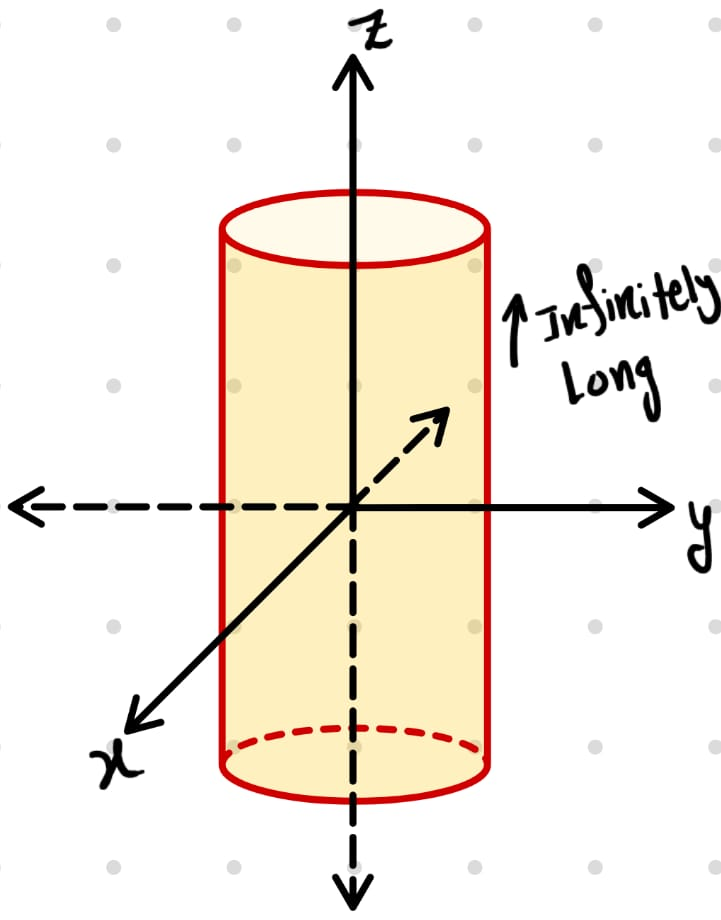
\includegraphics[width=0.3\textwidth]{Images/infinite_sol1.jpeg}
\caption{}
\label{sol_pb1}
\end{figure}
Using this, 
\begin{equation*}
    \vec{K}\times \vec{\scriptr} = K \cos(\theta)\, z' \hat{x} - K \sin(\theta)\, z' \hat{y} + (K\sin(\theta)(R\sin(\theta)-y)+K\cos(\theta)(R\cos(\theta)-x))\hat{z}
\end{equation*}
The differential area,
\begin{equation*}
    d^2r' = R\, d\theta \, dz'
\end{equation*}
Hence, we have,
\begin{equation}
    B_z = \frac{\mu_0}{4\pi}\int_{\infty}^{\infty}\frac{(K\sin(\theta)(R\sin(\theta)-y)+K\cos(\theta)(R\cos(\theta)-x))}{[(x-R\cos(\theta)^2+(y-R\sin(\theta))^2+ z'^2)]}R\, d\theta dz'
\end{equation}
There will be no $B_x$ and $B_y$ as the integrations are odd in $x$ and $y$ for those.
This if done (with contour integration) will gives us,
\begin{equation}
\begin{split}
    \vec{B} &= \mu_0 K \hat{z}\, \,  \text{inside}\\
    &= 0 \, \, \text{outside}
\end{split}
\end{equation}
\subsection{Potentials}
Will update later
\lecture{Green's Theorem and Integral form of Potential}
\subsection{Introduction}
As discussed previously, Harmonic Functions are sort of average. To see this, let's see this:\\
In the fig-\ref{sp_av_cen}, there is a charge $q$ at a distance $z$ and a spherical surface of radius $R$ close to it. The potential at a point on the sphere is,
\begin{equation*}
    V(\vec{r})=V = \frac{1}{4\pi \epsilon_0}\frac{q}{\scriptr}
\end{equation*}
Here $\scriptr$ can be written as $\scriptr^2=z^2 + R^2 -2\, R\, z \cos(\theta)$, where $\theta$ is the angle between the z axis and $d\vec{s}$ differential area. Then,
\begin{equation}
    \begin{split}
        \langle V\rangle = & \frac{\int_S V(s)\, ds}{\int_S \,ds}\\
                        = & \frac{1}{4\pi R^2}\int_S \frac{q}{4\pi \epsilon_0} \frac{R^2 \sin(\theta)\, d\theta \, d\phi}{(R^2 + z^2 -2R\, z \, \cos(\theta))^{1/2}}\\
                        = & \frac{q}{8\pi \epsilon_0}\int_{\theta = 0}^{\pi} \frac{\sin(\theta\, d\theta)}{(\lambda^2 - 2R\, z\, \cos(\theta))^{1/2}}
    \end{split}
\end{equation}
where $\lambda^2=R^2+z^2$. Now using the substitution $\lambda^2-2\, R\, z\, \cos(\theta)=y^2$, we ge,
\begin{equation}
    \langle V\rangle = \frac{q}{4\pi \epsilon_0 \, z}
\end{equation} 
\begin{figure}[H]
\centering
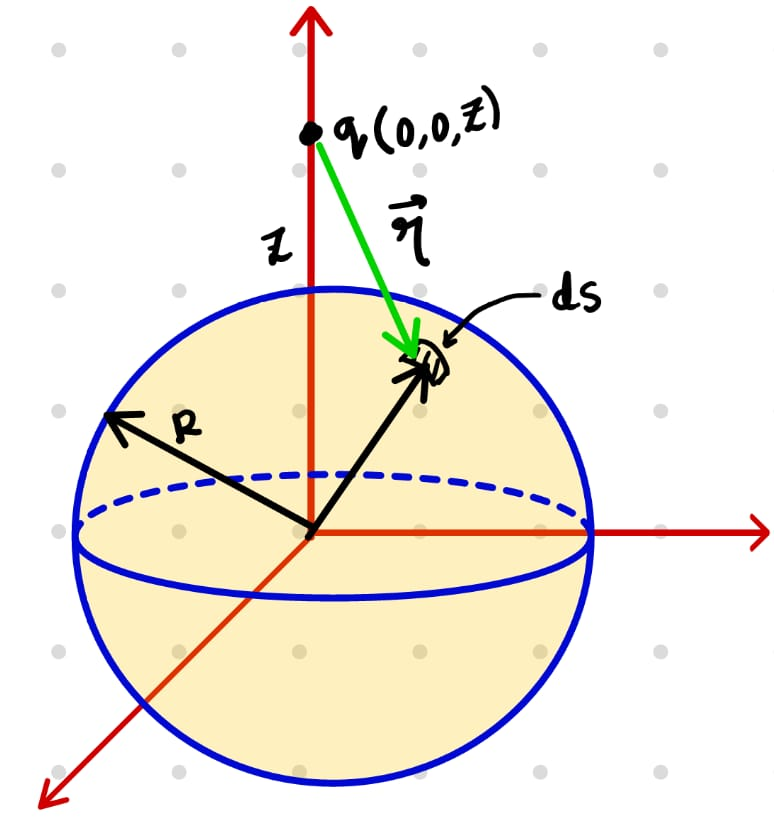
\includegraphics[width=0.3\textwidth]{Images/sp_av_cen.jpeg}
\caption{}
\label{sp_av_cen}
\end{figure}
This is exactly the potential due to $q$ at the center of the sphere. By the superposition principle, the same will happen for any collection of charges outside the sphere. So, It doesn't matter if \textbf{our region of interest is charge-less and there are other charges outside that region, we will just get an average potential due to all other charges at the center of the region}.

This again implies \textcolor{red}{\textbf{The soln to the laplace equation doesn't admit local maxima or minima}}.

Laplace's Equation doesn't by itself determines $V$ like mentioned already. Along with it we need some suitable set of boundary conditions. This naturally creates a very serious question: \textcolor{blue}{\textbf{What are appropriate boundary conditions, sufficient to determine the potential but not so strong as to generate inconsistencies}}?\\
The idea that some set of boundary conditions will suffice is usually presented in the form of a \textbf{Uniqueness Theorem}. 

We have to understand that if electrostatic problems always involved localized discrete or continuous distribution of charge with no boundary surface, the general solution,
\begin{equation}
    V(\vec{r})=\int_{\mathcal{V}} \frac{\rho(\vec{r}')}{|\vec{r}-\vec{r}'|}\, d^3r'
    \label{pot_estat_g}
\end{equation}
would be the most convenient and straightforward solution of any problem. There would be no need of Poisson's or Laplace's equation. But many, if not most of the problems of electrostatics involve finite region of space, with or without charge inside, and with prescribed boundary conditions on the bounding surfaces. \textbf{For the solution of this boundary-value problem we need \textcolor{red}{Green's Theorem}}.
\subsection{Green's Theorem}
Let's say $\vec{A}$ is some vector field. We now from divergence theorem,
\begin{equation}
    \int_{\mathcal{V}}\nabla\cdot \vec{A}\, d^3r = \int_{\mathcal{\partial V}}\vec{A} \hat{n}\, d^2r
\end{equation}
Also let's assume $\psi_1(\vec{r}$ and $\psi_2(\vec{r}$ are two scalar fields and $\vec{A}=\psi_1(\vec{r})\nabla\psi_2(\vec{r})$. From the product rule,
\begin{equation}
    \nabla \cdot \vec{A} = \nabla \cdot (\psi_1(\vec{r})\nabla\psi_2(\vec{r}))=\psi_1 \nabla^2 \psi_2 + (\nabla \psi_!)\cdot (\nabla \psi_2)
\end{equation}
Using this along with the fact $\vec{A}\cdot n = \psi_1 (\nabla \psi_2)\cdot \hat{n}=\psi_1 \frac{\partial \psi_2}{\partial n}$ (the derivative of the scalar field $\psi_2$ in the direction of the normal vector to the surface), we can have,
\begin{equation}
    \int_{\mathcal{V}} (\psi_1 \nabla'^2 \psi_2 + (\nabla' \psi_1)(\nabla' \psi_2))\, d^3 r' = \int_{\partial \mathcal{V}}\psi_1 \frac{\partial \psi_2}{\partial n'}\, d^2 r'
    \label{green_th_1}
\end{equation}
This is called \textcolor{purple}{\textbf{First Green's Theorem}}. Here, we have used $'$ as integration variable. It really doesn't matter as it's a dummy variable but physically we can think that as we will be working with source terms, we are using it (although really not).

The \textcolor{purple}{\textbf{Second Green's Theorem}} is found by interchanging the arbitrarily chosen scalar fields in eqn-\ref{green_th_1} and subsequent subtraction. This gives us,
\begin{equation}
    \int_{\mathcal{V}} (\psi_1 \nabla'^2 \psi_2 - \psi_2 \nabla'^2 \psi_1)\, d^3 r' = \int_{\partial \mathcal{V}}\Bigg(\psi_1 \frac{\partial \psi_2}{\partial n'} - \psi_2 \frac{\partial \psi_1}{\partial n'}\Bigg)\, d^2 r'
    \label{green_th_2}
\end{equation}
\subsection{Integral Equation of Potential}
From Green's theorem and employing Poisson's equation, we want to find an \textbf{integral representation of the potential more general than eqn-\ref{pot_estat_g}}. That was the goal from the beginning. For this let's those arbitrary scalars as,
\begin{equation}
    \begin{split}
        \psi_1 = & \frac{1}{\scriptr} = \frac{1}{|\vec{r}-\vec{r}'|}\\
        \psi_2 = & V(\vec{r}')
    \end{split}
\end{equation}
Now, $\nabla^2 \psi_1 = -4\pi \delta^3(\vec{r}-\vec{r}')$. Hence, we have,
\begin{equation}
    \begin{split}
        \int_{\mathcal{V}} \Bigg(\frac{1}{|\vec{r}-\vec{r}'|} \nabla'^2 V(\vec{r}') + V(\vec{r}') \, 4\pi \delta^3(\vec{r}-\vec{r}')\Bigg)\, d^3 r' = & \int_{\partial \mathcal{V}}\Bigg(\frac{1}{|\vec{r}-\vec{r}'|} \frac{\partial V(\vec{r}')}{\partial n'} - V(\vec{r}') \frac{\partial |\vec{r}-\vec{r}'|^{-1}}{\partial n'}\Bigg)\, d^2 r'\\
        \to \int_{\mathcal{V}} \Bigg(\frac{1}{|\vec{r}-\vec{r}'|} \frac{(-\rho)}{\epsilon_0} + V(\vec{r}') \, 4\pi \delta^3(\vec{r}-\vec{r}')\Bigg)\, d^3 r' = & \int_{\partial \mathcal{V}}\Bigg(\frac{1}{|\vec{r}-\vec{r}'|} \frac{\partial V(\vec{r}')}{\partial n'} - V(\vec{r}') \frac{\partial |\vec{r}-\vec{r}'|^{-1}}{\partial n'}\Bigg)\, d^2 r'\\
    \end{split}
\end{equation}
If the \textcolor{blue}{\textbf{point of observation $\vec{r}$}} lies inside the integration volume, the second term of \gls{lhs} gives us $V(\vec{r})$ and rearranging a bit, we get,
\begin{equation}
    V(\vec{r}) = \frac{1}{4\pi \epsilon_0}\int_{\mathcal{V}}\frac{\rho(\vec{r}')}{\scriptr}\, d^3 r' + \int_{\partial \mathcal{V}}\Bigg(\frac{1}{\scriptr} \frac{\partial V(\vec{r}')}{\partial n'} - V(\vec{r}') \frac{\partial\frac{1}{\scriptr}}{\partial n'}\Bigg)\, d^2 r'
    \label{pot_estat_gene}
\end{equation}
\begin{equation}
    \langle V\rangle = \frac{q}{4\pi \epsilon_0 \, z}
\end{equation} 
We can study this last expression in two special cases.
\begin{enumerate}
    \item We shift the integration surface $\partial\mathcal{V}$ to infinity. Then, the integral goes faster to zero (eg: for a point charge)
    \begin{equation*}
        \frac{1}{\scriptr}\frac{\partial V}{\partial n'}\sim \frac{1}{\vec{r}'^3}
    \end{equation*}
    than the surface element tends to infinity. This results in,
    \begin{equation*}
        V(\vec{r}) = \int_{\mathcal{V}} \frac{\rho(\vec{r}')}{|\vec{r}-\vec{r}'|}\, d^3r'
    \end{equation*}
    which is exactly eqn-\ref{pot_estat_g}
    \item If the integration volume $\mathcal{V}$ is free of charge, $\rho = 0$ and the potential is determined only by the values of the \textbf{potential} and it's \textbf{derivative at the boundary $\partial\mathcal{V}$}. 
\end{enumerate}
One should note that the integration volume always has to contain the point $\vec{r}$ in order to get a solution for the potential. The eqn-\ref{pot_estat_gene} is just a solution in integral form just like we see in Dyson series in perturbation theory of QM.

We can use an iterative method to actually solve this just like we do for dyson series.
\begin{note}
    Eqn-\ref{pot_estat_gene} is consistent with the interpretation of the surface integral as being the potential due to a surface charge density(induced by other charges outside $\mathcal{V}$) $\sigma = \frac{\partial V}{\partial n'}$ and a dipole layer $D=-V$.
\end{note}
\lecture{Evaluation of Potentials: Boundary Conditions, Uniqueness and Green's Function}
From eqn-\ref{pot_estat_gene} the potential $V(\vec{r})$ is determined by the potential and it's normal derivative on the boundary surface. But, by giving both values $V(\partial \mathcal{V})$ and $\frac{\partial V}{\partial n}|_{\partial \mathcal{V}}$ the problem is overdetermined. We can show that \textcolor{purple}{\textbf{it is enough to give one condition to fix the potential}}.\\
\textcolor{blue}{\textbf{The boundary conditions are called \gls{dbc} if $V$ is given at the boundary}} and \textcolor{blue}{\textbf{\gls{nbc} if $\partial V/\partial n$ is given at the boundary}}.

It can be proven very easily. Let's see:
\subsection{Proof of Dirichlet and Neumann Boundary Condition}
Suppose, there are two solutions $V_1(\vec{r})$ and $V_2(\vec{r})$ of the Poission Equation (or Laplace Equation),
\begin{equation}
    \nabla^2 V_{1,2}(\vec{r}) = -\frac{\rho(\vec{r})}{\epsilon_0} \implies \nabla^2 (V_1 -V_2) = 0
\end{equation}
At the boundary both functions satisfy the same conditions, i.e.,
\begin{equation}
    V_1(\partial \mathcal{V}) = V_2(\partial \mathcal{V}) \text{ \ \ or \ \ } \frac{\partial V_1}{\partial n}\Bigg|_{\partial \mathcal{V}} = \frac{\partial V_2}{\partial n}\Bigg|_{\partial \mathcal{V}}
\end{equation}
Now setting $u=V_1 - V_2$ and using $\psi_1=\psi_2=u$ in eqn-\ref{green_th_1},  we will have,
\begin{equation}
\begin{split}
    \int_{\mathcal{V}} \Bigg [ u(\vec{r}')\nabla'^2u(\vec{r}') + (\nabla'u(\vec{r})')^2 \Bigg]\, d^3r' =& \int_{\partial \mathcal{V}} u(\vec{r}')\frac{\partial u}{\partial n}\, d^2r'\\
    \implies \int_{\mathcal{V}}  (\nabla'u(\vec{r})')^2 \, d^3r' =& \int_{\partial \mathcal{V}} u(\vec{r}')\frac{\partial u}{\partial n}\, d^2r
\end{split}
\end{equation}
The surface integral becomes $0$ since either $u$(\gls{dbc}) or $\partial u/\partial n$(\gls{nbc}) vanish on the surface due to the boundary conditions. This gives,
\begin{equation}
     \int_{\mathcal{V}}  (\nabla'u(\vec{r})')^2 \, d^3r' = 0 \implies \nabla'u(\vec{r}')=0
\end{equation}
Thus, $u$ \textbf{is constant throughout the volume $\mathcal{V}$}. Hence,
\begin{enumerate}
    \item For \gls{dbc}, $u$ is $0$ at the boundary and we have $u=0$ everywhere, i.e., $V_1=V_2$. Hence, Uniqueness.
    \item For \gls{nbc}, both $V_1$ and $V_2$ differ at most in some additive constant, which for potential doesn't matter as we can always shift the zero-level. Hence, again Uniqueness.
\end{enumerate}
\begin{note}
If both value of potential and it's derivative is given then it's \textbf{Cauchy Boundary Condition}, which in our case will be overspecified. But in general for any PDE it's not so. Here is a table to give a brief overview on this.
\begin{table}[H]
\centering
\small % Reduce font size
\renewcommand{\arraystretch}{1.4}
\setlength{\tabcolsep}{4pt} % reduce padding
\begin{tabular}{|p{3.2cm}|p{3.5cm}|p{3.5cm}|p{5cm}|}
\hline
\textbf{Type of Boundary Condition} & 
\textbf{Elliptic (Poisson’s eq.)} & 
\textbf{Hyperbolic (wave eq.)} & 
\textbf{Parabolic (heat-conduction eq.)} \\
\hline
\textit{Dirichlet} Open surface & Not enough & Not enough & \colorbox{faintpink}{Unique, stable in one direction} \\
\hline
\textit{Dirichlet} Closed surface & \colorbox{faintpink}{Unique, stable solution} & Too much & Too much \\
\hline
\textit{Neumann} Open surface & Not enough & Not enough & \colorbox{faintpink}{Unique, stable in one direction} \\
\hline
\textit{Neumann} Closed surface & \colorbox{faintpink}{Unique, stable in general} & Too much & Too much \\
\hline
\textit{Cauchy} Open surface & Unphysical results & \colorbox{faintpink}{Unique, stable solution} & Too much \\
\hline
\textit{Cauchy} Closed surface & Too much & Too much & Too much \\
\hline
\end{tabular}
\caption{Boundary condition requirements for different PDE types.}
\label{tab:boundary_conditions}
\end{table}
\end{note}
But the question is how exactly can we be sure that we can remove $V$ or derivative of it without any issue? That's hidden an additional degree of freedom of this theory. We will see that in the discussion below.
\subsection{Green's Function}
Now, we know we need either the potential value at bounding surface or it's normal to get unique solution but still eqn-\ref{pot_estat_gene} is a integral-solution. We still don't have any actual solution. Let's change that by using the \textbf{Green's Theorem} along with \textcolor{purple}{\textbf{Green's Function}}.
\begin{note}
    Consider a general linear second order differential equation $\mathcal{L}$ on $[l,m]$. We can write it as,
    \begin{equation*}
        \mathcal{L}y(x) = a(x)\frac{d^2y}{dx^2} + b(x) \frac{dy}{dx} + c(x) = f(x)
    \end{equation*}
    where $a,b,c$ are continuous functions on $[l,m]$ and $a$ is nonzero(maybe at some finite number of isolated points it can also be $0$). Then, Green's function $G(x,\xi)$ of $\mathcal{L}$ is a unique solution to the problem,
    \begin{equation*}
        \mathcal{L}G=\delta(x-\xi)
    \end{equation*}
    that satisfies homogeneous boundary conditions $G(l,\xi)=G(m,\xi)=0$. The beauty of this function is that, once we have this function, we can write the solution of $\mathcal{L}$ as,
    \begin{equation*}
        y(x) = \int_l^m G(x,\xi) f(\xi)\, d\xi
    \end{equation*}
    This exact thing we are going to use in our case.
\end{note}
See we have previously used $\psi_1=1/(\vec{r}-\vec{r}')$, Was there any reason to do that? Absolutely!

That is exactly the \textcolor{purple}{\textbf{potential of a unit point charge}}(apart from some factor). Hence, it satisfies as expected, 
\begin{equation*}
    \nabla'^2 \psi_1 = \nabla'^2\Bigg( \frac{1}{|\vec{r}-\vec{r}'|} \Bigg) = -4\pi \delta^3(\vec{r}-\vec{r}')
\end{equation*}
Interesting no?, This means it's basically the \textbf{Green's Function} of $\nabla'^2$ and we have chosen it from our intuition that delta-function is basically like charge distribution of point charge. So, We have,
\begin{equation}
    \nabla^2 G(\vec{r},\vec{r}') = -4\pi \delta(\vec{r}-\vec{r}')
\end{equation}
where,
\begin{equation}
    G(\vec{r},\vec{r}') = \frac{1}{|\vec{r}-\vec{r}'|} + \lambda(\vec{r},\vec{r}')
    \label{green_form1}
\end{equation}
With the function $\lambda$ must satisfy,
\begin{equation}
    \nabla'^2 \lambda(\vec{r},\vec{r}')=0
\end{equation}
Now, using eqn\ref{green_th_2}, with $\psi_1=V$ and $\psi_2=G(\vec{r},\vec{r}')$, we get,
\begin{equation}
    \begin{split}
        \int_{\mathcal{V}}\Bigg[ V(\vec{r}')\nabla'^2 G(\vec{r},\vec{r}') - G(\vec{r},\vec{r}') \nabla'^2 V(\vec{r}') \Bigg]\, d^3 r' = & \int_{\partial \mathcal{V}}\Bigg[ V(\vec{r}')\frac{\partial G}{\partial n'} - G(\vec{r},\vec{r}')\frac{\partial V}{\partial n'} \Bigg] \, d^2 r'\\
        \to \int_{\mathcal{V}}\Bigg[ V(\vec{r}')(-4\pi \delta^3(\vec{r}-\vec{r}')) - G(\vec{r},\vec{r}') \frac{-\rho(\vec{r}')}{\epsilon_0} \Bigg]\, d^3 r' = & \int_{\partial \mathcal{V}}\Bigg[ V(\vec{r}')\frac{\partial G}{\partial n'} - G(\vec{r},\vec{r}')\frac{\partial V}{\partial n'} \Bigg] \, d^2 r'\\
        \to  -4\pi\,V(\vec{r}) + \int_{\mathcal{V}}\Bigg[G(\vec{r},\vec{r}') \frac{-\rho(\vec{r}')}{\epsilon_0} \Bigg]\, d^3 r' = & \int_{\partial \mathcal{V}}\Bigg[ V(\vec{r}')\frac{\partial G}{\partial n'} - G(\vec{r},\vec{r}')\frac{\partial V}{\partial n'} \Bigg] \, d^2 r'\\
        \to V(\vec{r}) = \frac{1}{4\pi \epsilon_0}\int_{\mathcal{V}}G(\vec{r},\vec{r}')\rho(\vec{r}')+\frac{1}{4\pi}&\int_{\partial \mathcal{V}}\Bigg[ G(\vec{r},\vec{r}')\frac{\partial V}{\partial n'} - V(\vec{r}')\frac{\partial G}{\partial n'} \Bigg] \, d^2 r'
    \end{split}
\end{equation}
Now, using the \textbf{freedom of choosing} $\lambda$, we can choose $G$ such that first or second surface term vanishes. So, we don't have to worry about the other term.

Let's see that,
\begin{enumerate}
    \item For \gls{dbc}, we use $G_D(\vec{r},\vec{r}') = 0$ at $\vec{r}'$ on boundary $\partial \mathcal{V}$. Then, the equation becomes,
    \begin{equation*}
        V(\vec{r}) = \frac{1}{4\pi \epsilon_0}\int_{\mathcal{V}}G_D(\vec{r},\vec{r}')\rho(\vec{r}') - \frac{1}{4\pi} \int_{\partial \mathcal{V}}V(\vec{r}')\frac{\partial G_D}{\partial n'} \, d^2 r'
    \end{equation*}
    See now we only have $V$ on the boundary and that's what we need. We don't even have to worry about the other term.
    \item For \gls{nbc}, we can think obviously we should choose $\partial G_N/\partial n' = 0$ but this choice violates Gauss's law as,
    \begin{equation*}
        \int_{\partial \mathcal{V}}\frac{\partial G_N}{\partial n'}\, d^2 r' = -4\pi
    \end{equation*}

    A little thought tells us to choose, It as,
    \begin{equation}
        \frac{\partial G_N}{\partial n'}=-\frac{4\pi}{A}
    \end{equation}
    Where $A$ is the entire surface area and $\vec{r}'$ lies on the surface. Then we get,
    \begin{equation*}
    \begin{split}
        V(\vec{r}) =&  \frac{1}{4\pi A} \int_{\partial \mathcal{V}}V(\vec{r}')\, d^2r' +\frac{1}{4\pi \epsilon_0}\int_{\mathcal{V}}G_N(\vec{r},\vec{r}')\rho(\vec{r}') + \frac{1}{4\pi} \int_{\partial \mathcal{V}}\frac{\partial V}{\partial n'}G_N(\vec{r},\vec{r}') \, d^2 r'\\
         =& \langle V \rangle_{\partial \mathcal{V}} +\frac{1}{4\pi \epsilon_0}\int_{\mathcal{V}}G_N(\vec{r},\vec{r}')\rho(\vec{r}') + \frac{1}{4\pi} \int_{\partial \mathcal{V}}\frac{\partial V}{\partial n'}G_N(\vec{r},\vec{r}') \, d^2 r'
    \end{split}
    \end{equation*}
\end{enumerate}
I guess now we understand what exactly $\lambda$ does right?, It adjust the value of $G$. This $\lambda(\vec{r},\vec{r}')$ solves the Laplace's equation inside $\mathcal{V}$. Hence, the function $\lambda(\vec{r},\vec{r}')$ denotes the potential of a charge distribution outside the volume $\mathcal{V}$ so that \textcolor{purple}{\textbf{together with the potential $1/\scriptr$ of the point charge at the point $\vec{r}'$, the Green's Function can just reach the value $G_D(\vec{r},\vec{r}')=0$ or $\partial G_N/\partial n' = -4\pi/A$ at the boundary $\partial \mathcal{V}$}}
\begin{figure}[H]
\centering
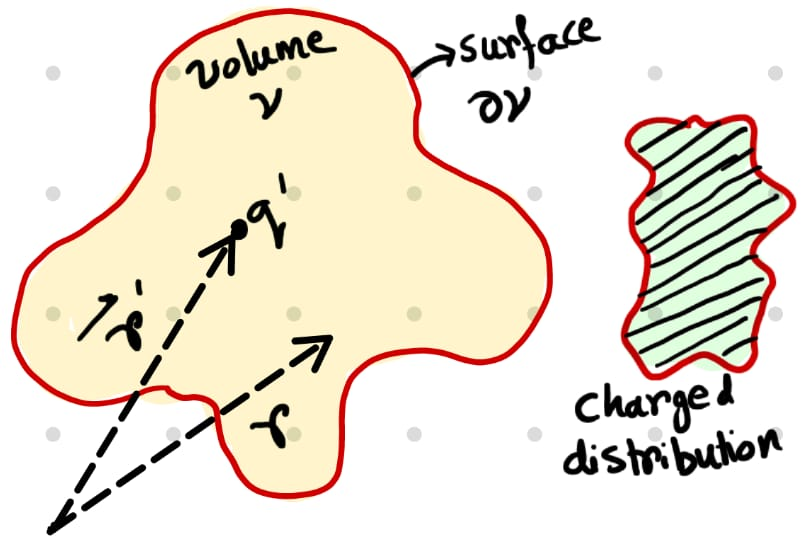
\includegraphics[width=0.4\textwidth]{Images/bound_dia_green1.jpeg}
\caption{The hatched region shows the charge distribution outside the volume $\mathcal{V}$ generating the \textbf{image potential} $\lambda(\vec{r},\vec{r}')$. Depending on where $q'$ lies in $\mathcal{V}$, that is, depending on $r$ , the image charge $\lambda(\vec{r},\vec{r}')$ will be different.}
\label{bound_dia_green1}
\end{figure}
It is clear that the external charge distribution depends on the point charge in the volume whose potential or the normal derivative of whose potential it has to compensate for at $\partial \mathcal{V}$. This is why we have chosen $\lambda$ to be a function of parameter $r'$, which gives the position of the point charge distribution in the volume. This is sort of what we do in Method of Images(see fig-\ref{bound_dia_green1}).
\subsection{Finding Green's Function for Grounded Conducting sphere image problem}
Let's see the problem of perfectly conducting sphere under method of images to see the the working of the things we discussed.


Consider a conducting sphere of radius $R$ held at ground potential ($V = 0$). Grounded means that the potential is the same as that of the surface of the earth, and therefore, the same as very far from the sphere, at $\infty$.
    \begin{figure}[H]
\centering
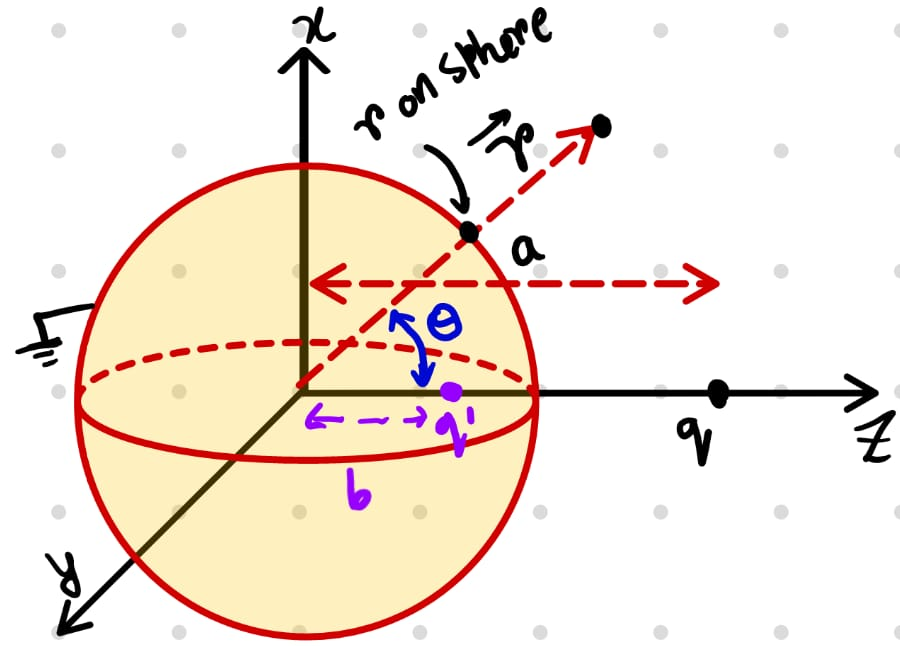
\includegraphics[width=0.4\textwidth]{Images/sph_imag_1.jpeg}
\caption{}
\label{met_img1}
\end{figure}
A charge $q$ is kept at a distance $a$ from the sphere's origin. We have chosen the $z$ axis so that the charge $q$ lies on it. $\vec{r}$ is the position of the point of interest(point of observation). We also know (i.e., boundary condition),
\begin{equation}
    V(R) = V(|\vec{r}|\to \infty) = 0
\end{equation}
This means we have to use \gls{dbc}. We will first use \textbf{method of images} to find $G_D$. Let's say it is at a distance $b$ from the origin inside the sphere with charge $q'$. The question is why inside? The reason is \textcolor{purple}{\textbf{That region is not our region of interest. So, that is the only region we can change such that boundary condition nor the region of interest changes}}. Due to symmetry $q'$ and $q$ will be on the same line. So, potential at $\vec{r}$ becomes,
\begin{equation}
    V(\vec{r},\hat{z}) = \frac{1}{4\pi \epsilon_0}\Bigg( \frac{q}{|\vec{r}-\vec{a}|} - \frac{q'}{|\vec{r}-\vec{b}|}\Bigg)
\end{equation}
This is function of position and angle with the $\vec{r}$ and z-axis, i.e., $\theta$. Now, on the surface this becomes,
\begin{equation*}
\begin{split}
    V(|\vec{r}|=R,\theta) =& \frac{1}{4\pi \epsilon_0}\Bigg( \frac{q}{(R^2+a^2-2R a\cos(\theta))^{1/2}} - \frac{q'}{(R^2+b^2-2R b\cos(\theta))^{1/2}}\Bigg)\\
    =& \frac{1}{4\pi \epsilon_0}\Bigg( \frac{q}{R(1+(a/R)^2-2(a/R)\cos(\theta))^{1/2}} - \frac{q'}{b(1+(R/b)^2-2 (R/b)\cos(\theta))^{1/2}}\Bigg) = 0
\end{split}
\end{equation*}
It is $0$ due to the boundary condition. Now, we can clearly see for it to hold, we must have,
\begin{equation}
    \begin{split}
        \frac{q}{R} &= -\frac{q'}{b} ; \frac{a}{R} = \frac{R}{b}\\
        \implies q' &= -\frac{b}{R}q ; b = \frac{R^2}{a}\\
        \implies q' &= -\frac{R}{a}q
    \end{split}
\end{equation}
These expression shows as $a\to \infty$ both $b=0$ and $q'=0$ (in math there is something similar called Spherical Inversion).


As, we know only boundary condition is $V(R)=0$(\gls{dbc}), we need to set $G_D(\vec{r},\vec{r}')=0$ when $\vec{r}$ is on the surface. This actually gives us,
\begin{equation}
    V(\vec{r}) = \frac{1}{4\pi \epsilon_0}\int_{\mathcal{V}}G_D(\vec{r},\vec{r}')\rho(\vec{r}')-\frac{1}{4\pi}\int_{\partial \mathcal{V}}\Bigg[V(\vec{r}')\frac{\partial G_D}{\partial n'} \Bigg] \, d^2 r'
    \label{pot_green1}
\end{equation}
Now, as we know, 
\begin{equation}
    G_D(\vec{r},\vec{r}') = \frac{1}{|\vec{r}-\vec{r}'|} + \lambda(\vec{r},\vec{r}')
    \label{green_form1}
\end{equation}
But without knowing $\lambda$ we can't have general solution. But do we find $\lambda$?, We just know that we have to choose $\lambda$ such that, $V$ on surface is $0$.\\
Well, by using the fact (previously mentioned once) that $\lambda(\vec{r},\vec{r}')$ solves Laplace's equation and it denotes the potential of a charge distribution(at $\vec{r}'$) outside the volume $\mathcal{V}$ such that the boundary condition is satisfied. So, as in eqn-\ref{green_form1}, the first term represent the potential due to a charge of value $4\pi \epsilon_0$, $\lambda$ should be the potential due to some charge outside $\mathcal{V}$(for us $\mathcal{V}$ is the whole space volume outside the sphere). Now, inside the charge is,
\begin{equation*}
    q' = -\frac{R}{r'}q = -\frac{R}{r'}(4\pi \epsilon_0)
\end{equation*}
at $R^2/r'$. This gives us,
\begin{equation}
    \lambda(\vec{r},\vec{r}') = \frac{1}{4\pi \epsilon_0} \frac{-4\pi \epsilon_0 R}{r'|\vec{r} - (R^2/r'^2)\vec{r}'|}= -\frac{R}{r'|\vec{r} - (R^2/r'^2)\vec{r}'|}
\end{equation}
Giving us,
\begin{equation}
    G_D(\vec{r},\vec{r}') = \frac{1}{|\vec{r}-\vec{r}'|} -\frac{R}{r'|\vec{r} - (R^2/r'^2)\vec{r}'|}
\end{equation}
Now we can find the potential at any point,i.e.,
\begin{equation}
    V(\vec{r},\vec{r}') = \frac{q}{4\pi \epsilon_0}\Bigg( \frac{1}{|\vec{r}-\vec{r}'|} - \frac{R}{r'|\vec{r} - (R^2/r'^2)\vec{r}'|}\Bigg)
\end{equation}
Although for this problem it's really not needed.
\begin{note}
    There is another way to find the image charge location and value for this problem as mentioned in class.\\
    Normally for $\nabla^2 V=0$ we use separation of variables and in case of azimuthal symmetry we get,
    \begin{equation}
        V(r,\theta) = \sum_{l=0}^{\infty}\Bigg( A_l r^l + \frac{B_l}{r^{l+1}} \Bigg)P_l(\cos(\theta))
        \label{azi_pot_sym1}
    \end{equation}
    Here $P_l$ represent Legendre Polynomials.\\
    But in this case it's not so simple as $\rho \neq 0$. Let's see it in a different manner. We will use (idea similar to method of images). We will remove $q$ with $V(\infty)=0$ \& set $V(R)$ equals something such that the potential due to $q$ on surface is same but negative. Setting the potential to what you may ask?

    To find that let's find the potential due to $q$ on the sphere. For any point $(x,y,z)$ on sphere, $\scriptr$ is,
    \begin{equation*}
        \begin{split}
            \scriptr |_R =& |(x,y,z) - (0,0,a)|_{R}\\
            =& [R^2 \sin^2(\theta)\cos^2(\phi)+ R^2 \sin^2(\theta)\sin^2(\phi)+(R\cos(\theta)-a)^2]^{1/2}\\
             =& [R^2 + a^2 - 2aR\cos(\theta)]^{1/2}
        \end{split}
    \end{equation*}
    Hence, the potential on the surface after charge is removed should be,
    \begin{equation*}
    \begin{split}
            V(R,\theta) =& -\frac{q}{4\pi \epsilon_0 \scriptr}\Bigg|_{\scriptr=R}\\
            =& \frac{-q}{4\pi\epsilon_0[R^2 + a^2 - 2aR\cos(\theta)]^{1/2}}\\
            =& \frac{-q}{4\pi\epsilon_0 a[1 + (R/a)^2 - 2(R/a)\cos(\theta)]^{1/2}}
        \end{split}
    \end{equation*}
    We have taken $a$ as common as $a>R$ and also that is generating function of Legendre Polynomial. Hence, we have,
    \begin{equation}
        V(R,\theta) = -\frac{-q}{4\pi\epsilon_0 a}\Big[ \sum_l \Big(\frac{R}{a}\Big)^l P_l(\cos(\theta))\Big]
    \end{equation}
    Again using eqn-\ref{azi_pot_sym1} we know $A_l=0$ as at $r\to\infty$ $V\to 0$. Hence,
    \begin{equation*}
        V(R,\theta) = -\frac{-q}{4\pi\epsilon_0 a}\Big[ \sum_l \Big(\frac{R}{a}\Big)^l P_l(\cos(\theta))\Big] = \sum_{l}\Bigg( \frac{B_l}{R^{l+1}} \Bigg)P_l(\cos(\theta))
    \end{equation*}
    Using these and equating the coefficient of $P_l$'s, we have,
    \begin{equation*}
        -\frac{q}{4\pi \epsilon_0 a}\Bigg(\frac{R}{a}\Bigg)^l=\frac{B_l}{R^{l+1}}\implies B_l = -\frac{q}{4\pi \epsilon_0}\frac{R^{2l+1}}{a^{l+1}}
    \end{equation*}
    Now, $V(r,\theta)$ is given by,
    \begin{equation}
        V(r,\theta) = -\frac{q}{4\pi \epsilon_0}\sum_{l}\Bigg( \frac{R^{2l+1}}{(a\,r)^{l+1}} \Bigg)P_l(\cos(\theta)) = \frac{-qR/a}{4\pi \epsilon_0 r}\sum_{l}\Bigg( \frac{R^{2l}}{(a\,r)^{l}} \Bigg)P_l(\cos(\theta))
    \end{equation}
    which can be written as (assuming $b = R^2/a$ and $q'=-qR/a$),
    \begin{equation}
        V(r,\theta) = \frac{q'}{4\pi \epsilon_0}\sum_{l}\Bigg( \frac{b^{l}}{r^{l}} \Bigg)P_l(\cos(\theta)) = \frac{q'}{4\pi\epsilon_0 r[1 + (b/r)^2 - 2(b/r)\cos(\theta)]^{1/2}}
    \end{equation}
    which is exactly if we have a (image) charge at a distance $b$ with charge $q'$.
\end{note}
\subsection{Recap of Uniqueness Theorem}
Now, let's recap the uniqueness theorems (from Griffith),
\begin{theorem}{1st Uniqueness Theorem}{}
    The solution to Poisson's equation in some volume $\mathcal{V}$ is uniquely determined if $V$ is specified on the boundary $S$(or same as $\partial \mathcal{V}$). 
\end{theorem}
\begin{proof}
    To prove it, Let's say we have a region(see fig-\ref{griff_1st_unq}) and it's boundary (There can be also "islands" inside, so long as $V$ is specified on all their surfaces; also the outer boundary could be at infinity, where $V$ normally is taken to be $0$).
        \begin{figure}[H]
        \centering
        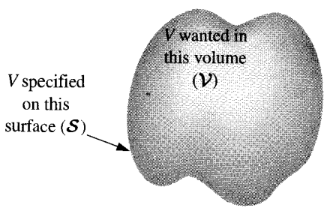
\includegraphics[width=0.4\textwidth]{Images/griff_1st_unq.png}
        \caption{}
        \label{griff_1st_unq}
        \end{figure}
    Suppose, there are two solutions to Poisson's equation,
    $$
    \nabla^2 V_1 = \frac{\rho}{\epsilon_0} \, ;\text{and}; \, \nabla^2V_2 = \frac{\rho}{\epsilon_0}
    $$
    Now, let's take $V_3 = V_1 - V_2$, this must solve,
    $$
    \nabla^2 V_3 = 0
    $$
    This has $0$ value on boundary \& as there are no local maxima and minima, maximum and minimum of $V_3$ both are $0$. Hence, $V_3$ must be $0$ everywhere, giving us $V_1=V_2$.
\end{proof}
\begin{theorem}{2nd Uniqueness Theorem}{}
    In a volume $\mathcal{V}$ surrounded by conductors and containing a specified charge density $\rho$, the electric field is uniquely determined if the total charge on each conductor is given(fig-\ref{griff_2nd_unq}).(The region as a whole can be bounded by another conductor or else unbounded)
\end{theorem}
\begin{proof}
    Suppose there are two fields satisfying the conditions of the problem. Both obey Gauss's law in differential form in the space between the conductors:
      $$
    \nabla \cdot \vec{E}_1 = \frac{\rho}{\epsilon_0} \, ;\text{and}; \, \nabla\cdot \vec{E}_2 = \frac{\rho}{\epsilon_0}
    $$
        \begin{figure}[H]
        \centering
        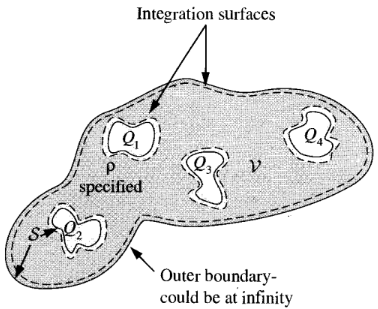
\includegraphics[width=0.4\textwidth]{Images/griff_2nd_unq.png}
        \caption{}
        \label{griff_2nd_unq}
        \end{figure}
    And both obey Gauss's law in integral form for a Gaussian Surface enclosing each conductor,
    \[
    \oint_{\text{i-conducting surface}} \vec{E}_1\cdot d\vec{a} \;=\; \frac{Q_1}{\epsilon_0}, \qquad
    \oint_{\text{i-conducting surface}} \vec{E}_2\cdot d\vec{a} \;=\; \frac{Q_2}{\epsilon_0}
    \]

    Likewise, for the outer boundary(whether this is just inside an enclosing conductor or at $\infty$),
    \[
    \oint\limits_{\text{outer boundary}} \vec{E}_1 \cdot d\vec{a} 
    = \frac{Q_{\text{tot}}}{\varepsilon_0},
    \qquad
    \oint\limits_{\text{outer boundary}} \vec{E}_2 \cdot d\vec{a} 
    = \frac{Q_{\text{tot}}}{\varepsilon_0}
    \]

    As before we can take $\vec{E}_3 = \vec{E}_1 - \vec{E}_2$ with the facts,
    \[
    \nabla \cdot \vec{E}_3 = 0 \ \ ; \ \ \oint\vec{E}_3\cdot d\vec{a}=0
    \]
    over each boundary.  Although, we don't know how the charge $Q_1$ distributes itself over the $i^{th}$ conducting surface.  We do know that each conductor is an equipotential and $V_3$ is a constant (not necessarily the same constant) over each conducting surface. 

    Now using,
    \begin{equation*}
        \nabla \cdot (V_3 \vec{E}_3) = V_3 (\nabla \cdot \vec{E}_3) + \vec{E}_3 \cdot (\nabla V_3) = -(E_3)^2
    \end{equation*}
    Integrating over the entire region between the conductors and applying divergence theorem,
    \begin{equation}
        \int_{\mathcal{V}}\nabla\cdot (V_3 \vec{E}_3)d\tau = \oint_S V_3 \vec{E}_3 \cdot d\vec{a} = -\int_\mathcal{V} E_3^2 d\tau
    \end{equation}
    The surface integral covers all boundaries of the region (the conductors and outer boundary). Now, $V_3$ is a constant over each surface(if the outer boundary is $\infty$, $V_3=0$ there), so it comes outside each integral, and what remains is $0$. Therefore,
    \begin{equation*}
        \int_{\mathcal{V}} E_3^2 d\tau = 0
    \end{equation*}
    But this integrand is never negative; the only way the integral can vanish is if $E_3=0$ everywhere. $\vec{E}_1=\vec{E}_2$ and the theorem is proved.
\end{proof}
Now, the question is does it only works for \textbf{scalar potential}? The answer is no!

% To see this, let's suppose for some region with (specific)\vec{J} in the interior or maybe $\vec{A}$ or $\vec{B}$ at the boundary is given. Then as before, $\vec{B}$ in the interior is uniquely specified.
% \begin{definition}{SpaceTime}{}
% SpaceTime is a 4D \textbf{Topological Manifold} with a smooth atlas carrying a \textbf{Torsion-Free} connection compatible with a \textbf{Lorentz Metric} and a \textbf{Time orientation} satisfying \textbf{Einstein's Field Equation}.
% \endexample

% \begin{minted}[mathescape,
%                linenos,
%                numbersep=5pt,
%                gobble=2,
%                frame=lines,
%                framesep=2mm]{csharp}
% u string title = "This is a Unicode π in the sky"
% /*
% Defined as $\pi=\lim_{n\to\infty}\frac{P_n}{d}$ where $P$ is the perimeter
% of an $n$-sided regular polygon circumscribing a
% circle of diameter $d$.
% */
% u const double pi = 3.1415926535
% \end{minted}

\end{document}
